\section*{Part 3 [68 points]}

\begin{enumerate}
    \item \textbf{[34 points]} Describe and analyze your hand-crafted policy. 
    \begin{enumerate}
    \item \textbf{[17 points]} With your scheduling policy, run the entire workflow \textbf{\textcolor{red}{3 separate times}}. For each run, measure the execution time of each batch job, as well as the latency outputs of memcached, running with a steady client load of 30K QPS. For each batch application, compute the mean and standard deviation of the execution time \footnote{Here, you should only consider the runtime, excluding time spans during which the container is paused.} across three runs. Also, compute the mean and standard deviation of the total time to complete all jobs - the makespan of all jobs. Fill in the table below. Finally, compute the SLO violation ratio for memcached for the three runs; the number of data points with 95th percentile latency $>$ 1ms, as a fraction of the total number of data points. The SLO violation ratio should be calculated during the time from when the first batch-job-container starts running to when the last batch-job-container stops running.  \\

        Create 3 bar plots (one for each run) of memcached p95 latency (y-axis) over time (x-axis), with annotations showing when each batch job started and ended, also indicating the machine each of them is running on. Using the augmented version of mcperf, you get two additional columns in the output: \texttt{ts\_start} and \texttt{ts\_end}. Use them to determine the width of each bar in the bar plot, while the height should represent the p95 latency. Align the $x$ axis so that $x=0$ coincides with the starting time of the first container. 
    For each core in each machine show what job it is running using the colors proposed in this template (you can find them in \texttt{main.tex}). For example, draw a bar in {\color{vips}the color of vips} for core x from when vips is started to when it ends if vips ran on core x.

    
    \textbf{Answer:} % Place your solution here.

% ────────────────────────────────────────────────────────────
\subsubsection*{Candidate screening methodology}
% ────────────────────────────────────────────────────────────

To limit cloud costs while exploring the design space, we designed
\textbf{5 candidate policies} and ran each one \emph{once} (screening run). \\
The policies were not picked at random: they sample a small, interpretable
design space tied to what we already measured in Part~1 and Part~2.
Part~1 showed that memcached tail latency reacts strongly to CPU and
last-level-cache pressure, which motivates (i) placing memcached on the
larger \texttt{node-a-8core} with a modest thread count, and (ii) treating
batch colocation with Memcached as an explicit lever - biasing toward isolation
by default, but still revisiting pairings when traces suggest net idle-time gain.
\\

Part~2a/2b supply parallel efficiency $E(8)$ and interference characterisations:
\texttt{radix} is the only strongly significant scaler ($E(8)=0.785$),
\texttt{streamcluster}, \texttt{barnes}, and \texttt{freqmine} are moderate,
and \texttt{blackscholes}, \texttt{canneal}, \texttt{vips} are weak at
8 threads. This motivates higher thread counts only for selected jobs near
memcached, while cache-/memory-heavy phases are either capped or isolated on
\texttt{node-b-4core}. \\

Against that background, \texttt{p01\_conservative\_isolation} stresses
maximum separation of cache-heavy batch work from node-a;
\texttt{p02\_balanced\_waves} uses paired waves (one batch job per physical node per wave) with moderate threads to avoid intra-node batch contention while keeping both worker nodes busy;

\texttt{p03\_cache\_aware\_staggered} and \texttt{p04\_aggressive\_parallel}
deliberately increase thread counts and overlap to hunt for shorter makespan at higher risk of oversubscription on the 4-core node;
\texttt{p05\_memcached\_guarded} tests keeping node-a as ``Memcached-first''
by moving the short \texttt{radix} phase to node-b.
Screening then filters out candidates that are infeasible on the Part~3
heterogeneous capacity regardless of these hypotheses. \\

\medskip
\noindent\textbf{From p02 baseline to final policy.}
\texttt{p02\_balanced\_waves} passed all gates and was initially selected as
the promoted policy. Three full runs produced makespans of 489\,s, 490\,s, and 520\,s.
Figure~\ref{fig:p3_p02_run1} shows a representative trace.

Inspecting the p02 Gantt charts revealed long idle periods on \texttt{node-b-4core}:
wave synchronization forces node-b to wait for \texttt{streamcluster} on node-a before
the next wave can start. This motivated two targeted follow-on experiments to reduce
barrier-induced idle time and shorten the makespan further.

We encoded two follow-on schedules as separate JSON policies for A/B comparison
against \texttt{p02}:
\begin{itemize}
  \item \texttt{p06\_longpair\_then\_shortpair}: \emph{no} change to which node
    hosts each job relative to \texttt{p02} - only the wave pairing changes.
    The middle waves become \texttt{streamcluster}$\parallel$\texttt{freqmine}
    and then \texttt{vips}$\parallel$\texttt{canneal}, instead of
    \texttt{streamcluster}$\parallel$\texttt{canneal} followed by
    \texttt{freqmine}$\parallel$\texttt{vips}, so the two long-running phases
    overlap across nodes instead of serializing on the short side.
  \item \texttt{p07\_shorttail\_radix\_last}: same Memcached placement and the
    same per-job thread counts as \texttt{p02}, but waves are reshaped:
    \texttt{blackscholes} moves from \texttt{node-b-4core} to
    \texttt{node-a-8core} to run alongside \texttt{barnes} (similar execution
    length in our traces), and the short \texttt{radix} job - which has no
    natural dual-node partner - is placed alone in the final wave.
    This adds batch traffic on \texttt{node-a-8core} versus \texttt{p02}, so it
    is not the conservative isolation pattern from \texttt{p01}; it is the same
    Part~1 trade-off (extra CPU/LLC pressure vs.\ barrier-induced idle) chosen
    because \texttt{blackscholes} is not among the LLC-heavy kernels we usually
    ban from node-a first (\texttt{barnes}, \texttt{freqmine}, \texttt{vips}).
    The gates below check that tail latency stays acceptable anyway.
\end{itemize}
These are not additional ``design-space corners'' like p01--p05; they are
deliberate reschedules suggested by the \texttt{p02} traces.

\begin{figure}[htbp]
    \centering
    
\includegraphics[width=0.8\textwidth]{Project Template/figures/part3a_run1.pdf}
    \caption{Representative \texttt{p02} run: memcached p95 latency (top) and per-core job placement on node-a/node-b (bottom panels).}
    \label{fig:p3_p02_run1}
\end{figure}

After the screening run we applied \textbf{four hard gates}:
\begin{itemize}
  \item \textbf{Validity gate}: all 7 PARSEC jobs must complete
    (no OOM / timeout / pod failure).

  \item \textbf{QPS-coverage gate}: $\geq 80\%$ of mcperf samples must fall
    in [29\,K, 31\,K]\,QPS during the batch window.

  \item \textbf{SLO gate}: fraction of near-30\,K samples with
    $\mathrm{p95} > 1\,\mathrm{ms}$ must be $\leq 1\%$.

  \item \textbf{Stability gate}: no continuous violation streak longer than
    60\,s.
\end{itemize}

Only policies passing all gates were promoted to 3 full runs.
This is sound for reporting because the final metrics come exclusively from the
3-run evaluation of the promoted policy.

Table~\ref{tab:screening} lists \textbf{seven} policy IDs (\texttt{p01}--\texttt{p07}):
the five initial screening candidates (\texttt{p01}--\texttt{p05}), plus two
follow-on wave-order experiments (\texttt{p06}, \texttt{p07}).  Among the
initial five, \texttt{p02\_balanced\_waves} was evaluated three times as the
baseline before \texttt{p06}/\texttt{p07}.

\begin{table}[htbp]
\centering
\small
\setlength{\tabcolsep}{6pt}
\renewcommand{\arraystretch}{1.15}

\caption{Screening and follow-on experiments. Policies p03--p05 failed
screening, while p02 and p07 were evaluated across three runs. Policy p06
was explored in a single run.}
\label{tab:screening}

\begin{tabular}{lccc p{5.2cm}}
\toprule
\textbf{Policy} & \textbf{Valid} & \textbf{Makespan [s]} &
\textbf{SLO} & \textbf{Key observation} \\
\midrule

p01\_conservative\_isolation
& Yes & 679 & 0\%
& Valid \texttt{run1\_old}, but slower than \texttt{p02}. \\

\textbf{p02\_balanced\_waves}
& Yes & 489 / 490 / 520 & 0\%
& Baseline policy; repeated idle periods on node-b due to wave synchronization. \\

p03\_cache\_aware\_staggered
& No & --- & ---
& Failed validity due to resource pressure / early abort. \\

p04\_aggressive\_parallel
& No & --- & ---
& Failed validity due to OOM and oversubscription on node-b. \\

p05\_memcached\_guarded
& No & --- & ---
& Failed validity because node-b became saturated. \\

p06\_longpair\_then\_shortpair
& Yes & 415 & 0\%
& Exploratory run pairing \texttt{streamcluster} with \texttt{freqmine}. \\

\textbf{p07\_shorttail\_radix\_last}
& Yes & 376 / 382 / 378 & 0\%
& \textbf{Selected configuration}; achieved the best average makespan. \\

\bottomrule
\end{tabular}
\end{table}

\noindent
Policies p03--p05 were discarded after a single run because the
\emph{validity gate failure was unambiguous}: fewer than 2 of 7 jobs
completed, which cannot be fixed by re-running --- it reflects a
fundamental resource-overcommitment in the policy specification.
Running two more repetitions would have wasted cluster time without
producing useful data.
Policy p01 was not promoted beyond screening because its makespan
(679\,s) was already much worse than the \texttt{p02} baseline, despite being
valid and SLO-safe in the retained \texttt{run1\_old} artifact.

Table~\ref{tabmakespancompare} compares batch \textbf{makespan only} across
\texttt{p02}, single-run \texttt{p06}, and three-run \texttt{p07}
(sources: \texttt{part3-screening/\{policy\}/run\{n\}/summary.json},
\texttt{makespan\_s}).

\begin{table}[htbp]
\centering
\small
\caption{End-to-end batch makespan (first batch container start $\to$ last
  batch container end): baseline \texttt{p02}, exploratory \texttt{p06},
  final \texttt{p07}.}
\label{tabmakespancompare}
\begin{tabular}{lrrrrr}
\toprule
\textbf{Policy} & \textbf{Run~1 [s]} & \textbf{Run~2 [s]} & \textbf{Run~3 [s]}
  & \textbf{Mean [s]} & \textbf{Std [s]} \\
\midrule
p02\_balanced\_waves           & 489 & 490 & 520 & 499.7 & 14.4 \\
p06\_longpair\_then\_shortpair & 415 & --- & --- & 415.0 & --- \\
p07\_shorttail\_radix\_last    & 376 & 382 & 378 & 378.7 & 2.5 \\
\bottomrule
\end{tabular}
\end{table}

Table~\ref{tab:p3_runtimes} expands the baseline \texttt{p02} row into
per-job container runtimes (same fields as in \texttt{summary.json}
\texttt{job\_times\_s}); steady mcperf load near 30\,K\,QPS.

\begin{table}[htbp]
\centering
\small
\caption{Batch-job execution times and makespan across 3 runs (policy
  \emph{p02\_balanced\_waves}).  Steady memcached load via mcperf scan near
  30\,K\,QPS.
  Values from \texttt{part3-screening/p02\_balanced\_waves/run\{n\}/summary.json}.}
\label{tab:p3_runtimes}
\begin{tabular}{lrrrrr}
\toprule
\textbf{Job} & \textbf{Run~1 [s]} & \textbf{Run~2 [s]} & \textbf{Run~3 [s]}
             & \textbf{Mean [s]} & \textbf{Std [s]} \\
\midrule
\texttt{barnes}        & 53 & 53 & 52 & 52.7 & 0.5 \\
\texttt{blackscholes}  & 47 & 46 & 48 & 47.0 & 0.8 \\
\texttt{canneal}       & 95 & 95 & 94 & 94.7 & 0.5 \\
\texttt{freqmine}      & 165 & 171 & 179 & 171.7 & 5.7 \\
\texttt{radix}         & 13 & 12 & 12 & 12.3 & 0.5 \\
\texttt{streamcluster} & 193 & 197 & 205 & 198.3 & 5.0 \\
\texttt{vips}          & 42 & 43 & 40 & 41.7 & 1.2 \\
\midrule
\textbf{Total makespan} & 489 & 490 & 520 & 499.7 & 14.4 \\
\bottomrule
\end{tabular}
\end{table}

Table~\ref{tab:p7_runtimes} is the same breakdown for the final policy
\texttt{p07\_shorttail\_radix\_last}.

\begin{table}[htbp]
    \centering
    \small
    \caption{Batch-job execution times and makespan across 3 runs
    (policy \emph{p07\_shorttail\_radix\_last}). Steady memcached load:
    30\,K\,QPS. All values are taken from \texttt{part3-screening/p07\_shorttail\_radix\_last/run\{n\}/summary.json}.}
    \label{tab:p7_runtimes}

    \begin{tabular}{ |c|c|c|c|c|c| }
        \hline
        job name & run 1 [s] & run 2 [s] & run 3 [s]
        & mean [s] & std [s] \\ \hline \hline

        \coloredcell{barnes}
            & 54  & 54  & 54  & 54.0  & 0.0 \\ \hline

        \coloredcell{blackscholes}
            & 46  & 51  & 46  & 47.7  & 2.4 \\ \hline

        \coloredcell{canneal}
            & 114 & 112 & 115 & 113.7 & 1.3 \\ \hline

        \coloredcell{freqmine}
            & 165 & 165 & 167 & 165.7 & 0.9 \\ \hline

        \coloredcell{radix}
            & 11  & 14  & 11  & 12.0  & 1.4 \\ \hline

        \coloredcell{streamcluster}
            & 151 & 152 & 166 & 156.3 & 6.9 \\ \hline

        \coloredcell{vips}
            & 40  & 55  & 39  & 44.7  & 7.3 \\ \hline

        total time
            & 376 & 382 & 378 & 378.7 & 2.5 \\ \hline
    \end{tabular}
\end{table}



    
\medskip
\noindent\textbf{Plots (final policy \texttt{p07\_shorttail\_radix\_last}).}

After observing the p02 traces and running follow-on experiments,
\texttt{p07\_shorttail\_radix\_last} was selected as the final policy.
Per-job runtimes across three runs are in Table~\ref{tab:p7_runtimes}.
The SLO violation ratio (fraction of 10-second mcperf intervals with
$\mathrm{p95} > 1\,\mathrm{ms}$ inside the batch window) was
\textbf{0/33 in run~1, 0/34 in run~2, and 0/34 in run~3}
(combined: $0/101 = 0.0\%$).



Figure~\ref{fig:p3a_three_plots} shows three stacked panels for
each \texttt{p07} run (generated from \texttt{mcperf\_1.txt} and
\texttt{pods\_1.json}; see \texttt{plot\_part3a.py}).

\begin{itemize}
  \item \emph{Top panel — p95 latency bar chart.}
    Each bar spans the mcperf interval (\texttt{ts\_start}–\texttt{ts\_end};
    $\sim$10\,s) and its height is p95 latency (µs columns converted to ms).
    Bar colour marks which batch job is active on \texttt{node-a-8core} at
    interval start.
    The \textbf{bottom strip} shows simultaneous node-b activity.
    The dashed line is the 1\,ms SLO.

    Across all three runs, p95 remains far below 1\,ms, consistent with the
    zero SLO-violation counts in \texttt{summary.json}.  Because wave~1 now
    places \texttt{blackscholes} on node-a, there is measurable co-location
    with memcached during that window; it remains within SLO for all runs.

  \item \emph{Middle / bottom panels — virtual-core Gantts.}
    Same convention as in the course template: virtual rows from thread
    counts and requests (no \texttt{taskset}); actual placement is OS-defined.

  \item \emph{Structural difference vs \texttt{p02}.}
    Pairing \texttt{streamcluster} with \texttt{freqmine} removes the long
    node-b idle stretch between \texttt{canneal} and \texttt{freqmine} that
    appeared under \texttt{p02}.  Finishing with a short \texttt{radix} wave
    replaces a long terminal \texttt{barnes}-only segment with a brief tail.
\end{itemize}

\begin{figure}[H]
    \centering

    \begin{subfigure}{0.49\textwidth}
        \centering
        
\includegraphics[width=\textwidth]{Project Template/figures/part3a_p07_run1.pdf}
        \label{fig:p3a_pol7_run1}
    \end{subfigure}
    \hfill
    \begin{subfigure}{0.49\textwidth}
        \centering
        
\includegraphics[width=\textwidth]{Project Template/figures/part3a_p07_run2.pdf}
        \label{fig:p3a_pol7_run2}
    \end{subfigure}

    \vspace{0.4cm}

    \begin{subfigure}{0.49\textwidth}
        \centering
        
\includegraphics[width=\textwidth]{Project Template/figures/part3a_p07_run3.pdf}
        \label{fig:p3a_pol7_run3}
    \end{subfigure}

    \caption{Three runs of \texttt{p07\_shorttail\_radix\_last}: memcached p95 latency (top) and per-core Gantt charts (bottom panels).}
    \label{fig:p3a_three_plots}
\end{figure}

Figure~\ref{fig:p3a_pol6_run1} shows the single \texttt{p06} run for comparison.
\begin{figure}[H]
    \centering
    
\includegraphics[width=0.49\textwidth]{Project Template/figures/part3a_p06_run1.pdf}
    \caption{Single run of \texttt{p06\_longpair\_then\_shortpair} (415\,s makespan).}
    \label{fig:p3a_pol6_run1}
\end{figure}

    \item \textbf{[17 points]} Describe and justify the “optimal” scheduling policy you have designed. 
    
    \begin{itemize}
        \item Which node does memcached run on? Why?

        \textbf{Answer:} \texttt{node-a-8core} (e2-standard-8).

Same rationale as before: larger LLC and mem bandwidth vs node-b; memcached
remains at \textbf{2 threads} (\texttt{-t~2}) with a 2~CPU \texttt{requests}
budget.

        \item Which node does each of the 7 batch jobs run on? Why?

        \textbf{Answer:}
        \begin{itemize}
            \item \colored{barnes}: node-b-4core
            
            \item \colored{blackscholes}: node-a-8core
            
            \item \colored{canneal}: node-b-4core
            
            \item \colored{freqmine}: node-b-4core
            
            \item \colored{radix}: node-a-8core
            
            \item \colored{streamcluster}: node-a-8core
            
            \item \colored{vips}: node-a-8core
        \end{itemize}

        \textbf{Why:} \texttt{freqmine}, \texttt{barnes}, and often \texttt{canneal} are cache/memory-bandwidth heavy in Part~2a; isolating them on node-b reduces interference risk on the latency path.  \texttt{streamcluster} and \texttt{radix} benefit from faster cores; \texttt{vips} stays at 2 threads for low L1I blast radius.

        \item Which jobs run concurrently / are colocated? Why?

        \textbf{Answer:} four waves, one batch job per node per wave (plus a final
node-a-only wave):
\begin{enumerate}
  \item Wave~1: \texttt{barnes} (node-b) $\|$ \texttt{blackscholes} (node-a)
  \item Wave~2: \texttt{freqmine} (node-b) $\|$ \texttt{streamcluster} (node-a)
  \item Wave~3: \texttt{canneal} (node-b) $\|$ \texttt{vips} (node-a)
  \item Wave~4: \texttt{radix} (node-a) alone
\end{enumerate}


        \item In which order did you run the 7 batch jobs? Why?
    
        \textbf{Order (node-a):}
        \colored{blackscholes} $\to$ \colored{streamcluster} $\to$ \colored{vips} $\to$ \colored{radix}.

        \textbf{Order (node-b):}
        \colored{barnes} $\to$ \colored{freqmine} $\to$ \colored{canneal}.

\textbf{Why:} the wave schedule pairs long work (\texttt{streamcluster} with
\texttt{freqmine}) to reduce barrier-induced idle time relative to
\texttt{p02}. \texttt{barnes} and \texttt{blackscholes} have similar runtimes (mean 52\,s and 47\,s). \texttt{radix} is last because it is the shortest job; it adds only a brief tail.



        \item How many threads have you used for each of the 7 batch jobs? Why?
    
        \textbf{Answer:}
    
        \begin{itemize}
            \item \colored{barnes}: 2 threads (node-b)
            \item \colored{blackscholes}: 2 threads (node-a)
            \item \colored{canneal}: 2 threads (node-b)
            \item \colored{freqmine}: 2 threads (node-b)
            \item \colored{radix}: 4 threads (node-a)
            \item \colored{streamcluster}: 4 threads (node-a)
            \item \colored{vips}: 2 threads (node-a)
        \end{itemize}

        \texttt{radix} and \texttt{streamcluster} use 4\,threads on node-a based on
        $E(8)$ tiers from Part~2. All node-b jobs are capped at 2\,threads:
        \texttt{p04} showed that $>2$\,t per job on node-b risks OOM under colocation.

        \item Which files did you modify or add and in what way? Which Kubernetes features did you use?
    
        \textbf{Answer:}
\begin{itemize}
  \item \textbf{Added} \texttt{run\_part3a.py} — automation script that
    reads a policy from \texttt{part3\_policies.json}, launches memcached
    and batch jobs via \texttt{kubectl apply}, and polls for wave completion
    before advancing.
  \item \textbf{Added} \texttt{part3\_policies.json} — JSON policy library
    defining node assignment, thread count, and wave order for all 7
    candidate policies.
  \item \textbf{Generated on-the-fly} — Kubernetes Job manifests (one per
    batch job) with \texttt{nodeSelector} and \texttt{resources.requests}.
  \item \textbf{Modified} \texttt{memcache-t1-cpuset.yaml} — updated to
    target node-a via \texttt{nodeSelector} and run with 2 memcached
    threads.
\end{itemize}

\textbf{Kubernetes features used:}
\begin{itemize}
  \item \texttt{nodeSelector} (label \texttt{cca-project-nodetype}) — pins
    each Job pod and the memcached Pod to the correct node.
  \item \texttt{resources.requests} — declares CPU and memory requirements
    so the Kubernetes scheduler can enforce admission control and avoid
    over-commitment.
  \item \texttt{batch/v1 Jobs} with \texttt{backoffLimit: 0} — batch
    semantics with immediate failure propagation.
  \item \texttt{NodePort Service} — exposes memcached on a predictable
    port for the mcperf clients outside the cluster.
\end{itemize}
    
        \item Describe the design choices, ideas and trade-offs you took into account while creating your scheduler (\underline{if not already mentioned above}). Describe how your policy (and its performance) compares to another policy that you experimented with (in particular to the second-best policy that you designed).

        \textbf{Answer:}\\
\textbf{Selected policy — \texttt{p07\_shorttail\_radix\_last}.}
It preserves the safe cross-node isolation model of \texttt{p02} while
reordering waves to directly attack the dominant barrier and tail-loss effects.
Mean makespan $\mathbf{378.7 \pm 2.5}$\textbf{\,s} with \textbf{0\%} SLO
violations over three runs.

\textbf{vs \texttt{p02}} (Table~\ref{tabmakespancompare}): mean batch window
shortens by $\approx 121$\,s ($\approx 24\%$) relative to the \texttt{p02}
mean, with comparable SLO behaviour.

\textbf{vs \texttt{p06}} (single exploratory screening run): \texttt{p06} also
passes gates at 415\,s but \texttt{p07} delivers lower mean makespan under three
repetitions and is therefore the reported design.

\textbf{Second-best reference — \texttt{p02\_balanced\_waves}.}
It is the original fully evaluated baseline with transparent wave structure and
clear identification of the node-b idle gap that motivated \texttt{p06} and
\texttt{p07}.

\textbf{vs \texttt{p01}} remains unchanged from the screening discussion: valid
but substantially slower.

    
    \end{itemize}
    \end{enumerate}
    \item \textbf{[34 points]} Describe and analyze the AI-generated policy.

    \begin{enumerate}
        \item \textbf{[17 points]} \textbf{Report the performance}:

        \begin{itemize}
            \item Report the mean time of each batch job, as well as the makespan of all jobs for the AI-generated policy. Also, report the SLO violation ratio for memcached for the AI-generated policy. \textit{Note: If the LLM failed to produce a valid solution after 3+ attempts, provide the error logs and your best-performing manual tweak for partial credit.}

        \noindent\textbf{AI-generated policy.}
        The final policy produced by OpenEvolve (\texttt{run\_26 / checkpoint\_5}) uses two waves:
        \begin{itemize}
          \item \textbf{Wave 1:} \texttt{streamcluster} (4 threads, node-a) $\parallel$ \texttt{freqmine} (2 threads, node-b) $\parallel$ \texttt{canneal} (2 threads, node-b).
          \item \textbf{Wave 2:} \texttt{blackscholes} (2, node-a) $\parallel$ \texttt{vips} (2, node-b) $\parallel$ \texttt{barnes} (2, node-a) $\parallel$ \texttt{radix} (4, node-a).
        \end{itemize}
        We ran the AI policy \textbf{4 times}; run 1 showed elevated runtimes due to cluster warm-up effects and is excluded from the mean. Runs 2--4 are used for statistical reporting below (mean $\pm$ std). The SLO violation ratio was \textbf{0.000} across all four runs. Baseline values are the mean over 3 runs of policy \texttt{p07\_shorttail\_radix\_last}.

        \begin{table}[ht]
            \centering
            \begin{tabular}{ |c|c|c|c|}
                \hline
                job name & mean [s] (Baseline \texttt{p07}) & mean [s] (AI, runs 2--4) & std [s] (AI) \\ \hline \hline
                \coloredcell{barnes}          & 54.0  & 101.3 & 1.5 \\  \hline
                \coloredcell{blackscholes}    & 47.7  & 106.7 & 0.6 \\  \hline
                \coloredcell{canneal}         & 113.7 & 109.0 & 0.0 \\  \hline
                \coloredcell{freqmine}        & 165.7 & 199.7 & 9.9 \\  \hline
                \coloredcell{radix}           & 12.0  &  20.0 & 1.0 \\  \hline
                \coloredcell{streamcluster}   & 156.3 & 242.3 & 3.1 \\  \hline
                \coloredcell{vips}            & 44.7  &  76.0 & 2.6 \\  \hline
                total time (makespan)         & 378.7 & 379.7 & 2.1 \\  \hline
            \end{tabular}
            \caption{Per-job execution times and makespan. Baseline = mean of 3 runs of \texttt{p07\_shorttail\_radix\_last}; AI = mean/std of runs 2--4 of the OpenEvolve best policy. SLO violation ratio = 0.000 for all runs.}
            \label{tab:ai_vs_baseline}
        \end{table}

    \item Create 3 bar plots (one for each run), for the final AI-generated policy, of memcached p95 latency (y-axis) over time (x-axis), with annotations showing when each batch job started and ended, also indicating the machine each of them is running on. Use the same method as described in the previous question to create the bar plots.

    \textbf{Answer:}
    The plots were generated with \texttt{plot\_part3a.py} (the same script used for the hand-crafted policy evaluation in Part~3a), invoked as:
    \begin{verbatim}
python3 plot_part3a.py --screening-subdir part3b_ai_best \
    --out-prefix part3b_ai \
    --suptitle "AI-generated policy (OpenEvolve best)"
    \end{verbatim}
    We used the Part~3a script without modification because it is validated and the output format is identical. The AI policy was benchmarked using the same \texttt{run\_part3a.py} automation (the same runner script used for the hand-crafted experiments), which writes \texttt{mcperf\_N.txt} and \texttt{pods\_N.json} files in the same format expected by the plotter. All four runs are shown in Figure~\ref{fig:p3b_ai_runs} (run~1 is included for completeness; runs~2--4 are used for statistics). p95 latency remains below the 1\,ms SLO in all runs.


            \begin{figure}[H]
                \centering

                \begin{subfigure}{0.49\textwidth}
                    \centering
                    
\includegraphics[width=\textwidth]{Project Template/figures/part3b_ai_run1.pdf}
                    \label{fig:ai_latency_run1}
                \end{subfigure}
                \hfill
                \begin{subfigure}{0.49\textwidth}
                    \centering
                    
\includegraphics[width=\textwidth]{Project Template/figures/part3b_ai_run2.pdf}
                    \label{fig:ai_latency_run2}
                \end{subfigure}

                \vspace{0.4cm}

                \begin{subfigure}{0.49\textwidth}
                    \centering
                    
\includegraphics[width=\textwidth]{Project Template/figures/part3b_ai_run3.pdf}
                    \label{fig:ai_latency_run3}
                \end{subfigure}
                \hfill
                \begin{subfigure}{0.49\textwidth}
                    \centering
                    
\includegraphics[width=\textwidth]{Project Template/figures/part3b_ai_run4.pdf}
                    \label{fig:ai_latency_run4}
                \end{subfigure}

                \caption{Four benchmark runs of the AI-generated policy (\texttt{OpenEvolve run\_26 / checkpoint\_5}): memcached p95 latency (top) and per-core Gantt charts (bottom panels). Makespans: 410\,s (run~1, warm-up), 382\,s, 379\,s, 378\,s (runs~2--4). p95 remains below the 1\,ms SLO throughout all runs.}
                \label{fig:p3b_ai_runs}
            \end{figure}

    \item Create two line plots (one for the p95 latency and one for SLO violations) showing policy performance over iterations.

    \textbf{Answer:}
Figure~\ref{fig:iter_slo} summarises p95 latency and SLO violations across all four benchmark runs of the final AI policy.

\begin{figure}[H]
    \centering
    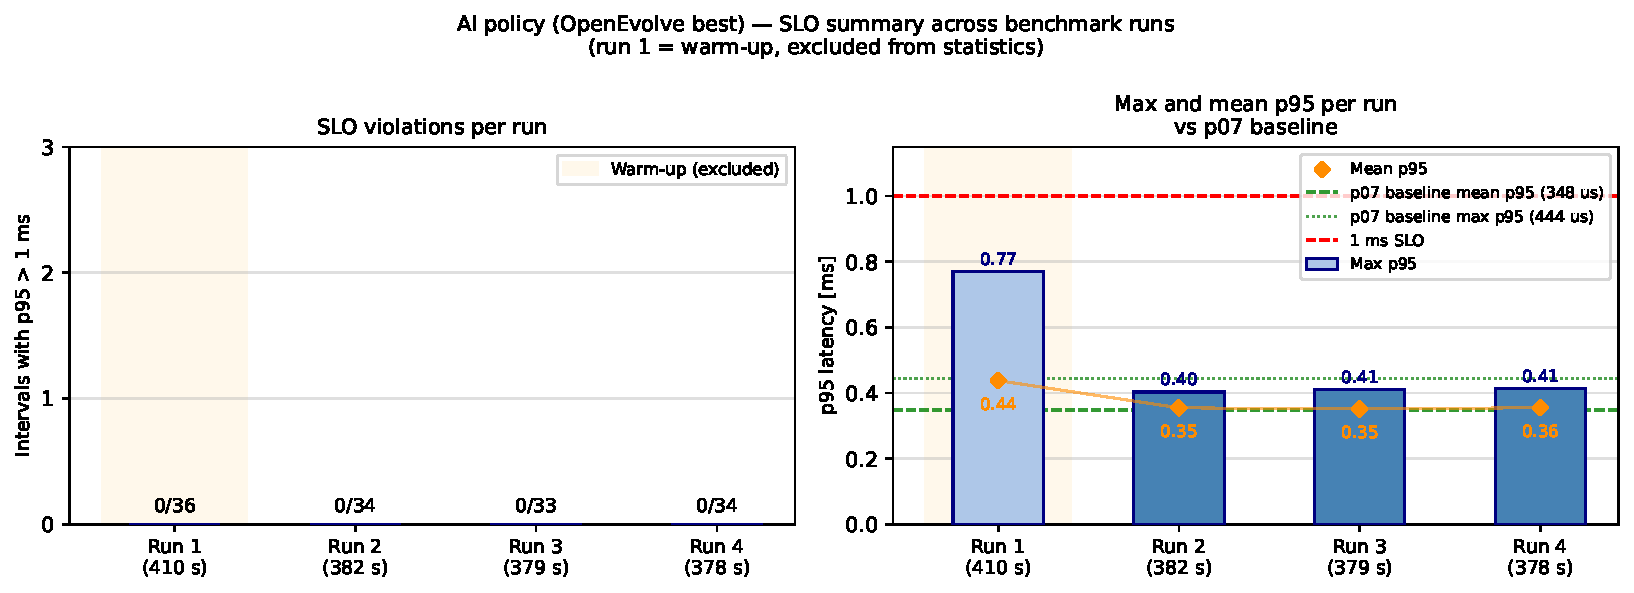
\includegraphics[width=\textwidth]{plots/part3b_iter_slo.pdf}
    \caption{Left: number of mcperf intervals with p95 $>$ 1\,ms per benchmark run (0 violations in all four runs). Right: maximum and mean p95 latency per run compared against the hand-crafted \texttt{p07} baseline. Maximum p95 stays well below 1\,ms (0.77\,ms worst case in the warm-up run~1; 0.41\,ms in runs~2--4). The \texttt{slo\_factor} inside OpenEvolve was non-functional due to the timestamp-mismatch bug described in Section~\ref{sec:ai_comparison}; actual SLO compliance is confirmed here from the raw mcperf data.}
    \label{fig:iter_slo}
\end{figure}

    \end{itemize}
    \item \textbf{[17 points]} Analysis of the Evolutionary Process: Describe the process of how you used OpenEvolve to design the AI-generated policy. For example, you can include the following details in your answer (You are not limited to these questions. You can include any other details you find relevant and interesting). Your response will be graded based on the thoroughness of the exploration and clarity in explanation:

        \begin{itemize}
            \item How many iterations did you run through OpenEvolve with the LLMs to get to the final policy? Which LLM(s) did you use?
            \item How do you measure success? For example, how do you design the `combined\_score' or the success metric, given that there are two objectives (makespan and SLO violations)?
            \item Describe the initial policy you fed to the LLM(s) and why you chose this as the initial policy.
            \item Describe how the policy changes during the process, and how it impacted the performance of the policy (e.g., tail latency; SLO violations).
            \item Explain why did this AI-generated policy perform better (or worse) than the baseline?
            \item Identify one ``hallucination'' or logical flaw the model produced during the process and how you identified it.
        \end{itemize}

         \textbf{Answer:}

\noindent\textbf{Setup and iterations.}
We ran \textbf{26 OpenEvolve runs} (named \texttt{run\_1}--\texttt{run\_26}), accumulating \textbf{77 checkpoint iterations} in total. All runs used the SwissAI CSCS inference endpoint (\texttt{api.swissai.cscs.ch}). Over the course of the experiment we tried \textbf{six different LLMs}:
\begin{itemize}
  \item \texttt{Qwen/Qwen3-Next-80B-A3B-Instruct-GICA} --- runs 3--7
  \item \texttt{meta-llama/Llama-3.3-70B-Instruct} --- runs 8--9, 17--19
  \item \texttt{swiss-ai/Apertus-70B-Instruct-2509} --- run 10
  \item \texttt{Qwen/Qwen3.5-27B} --- runs 11--16
  \item \texttt{Qwen/Qwen3.5-397B-A17B-NFgl} --- run 20
  \item \texttt{Qwen/Qwen2.5-Coder-14B-Instruct} --- runs 21--26 (final best policy)
\end{itemize}
The final best policy was produced by \texttt{Qwen2.5-Coder-14B-Instruct}. Switching models was motivated by the diversity collapse problem: when one model consistently reproduced the same output, we tried a different one in hopes of breaking the deadlock.

\medskip
\noindent\textbf{Success metric.}
We defined a two-objective combined score:
\[
  \text{combined\_score} = \text{makespan\_score} \times \text{slo\_factor}
\]
where $\text{makespan\_score} = \min(1,\; t_{\text{best}} / t_{\text{policy}})$ with $t_{\text{best}} = 378\,\text{s}$ (best hand-crafted makespan), and $\text{slo\_factor} \in \{0, 1\}$ acting as a hard gate: any p95 latency violation above 1\,ms sets \texttt{slo\_factor} to 0, capping the combined score at 0.  This multiplicative formulation means SLO compliance is a prerequisite for any makespan reward. The score is therefore bounded in $[0, 1]$, with 1.0 meaning the policy matched the hand-crafted best while keeping zero SLO violations.

\medskip
\noindent\textbf{Initial policy.}
We seeded OpenEvolve with the \texttt{p07\_shorttail\_radix\_last} hand-crafted policy (4 sequential waves, makespan $\approx 378\,\text{s}$). This was chosen as the initial policy because it already satisfied all hard constraints (freqmine/vips on node-b, canneal $\le$ 2 threads, no CPU overcommit), giving the LLM a valid and well-understood starting point rather than a blank slate.

\medskip
\noindent\textbf{Evolution process.}
The evolution was far more difficult in practice than the straightforward description above suggests. A large portion of total effort (over 20 of 26 runs) was spent \textbf{debugging the OpenEvolve harness and prompt engineering} rather than on productive policy search. The evolution can be divided into three phases.

\textit{Phase 1 --- diversity collapse (runs 1--23):} For the first 23 runs --- across six different LLMs --- every model produced output identical to the initial program in every checkpoint (\texttt{diversity = 0}). Each run looked superficially healthy: the evaluator returned a non-zero score, logs showed no errors, and checkpoints were written. Only by inspecting the actual \texttt{best\_program.py} files and comparing them byte-by-byte did we realize that every single generated program was a verbatim copy of the seed policy. The problem had two compounding causes:
\begin{itemize}
  \item \emph{Sampling configuration:} the original config used \texttt{temperature: 0.35} and \texttt{top\_p: 0.7}. At this entropy level, every model collapsed to a single greedy output --- effectively copying the most likely token sequence, which was the input itself.
  \item \emph{Missing evolutionary context:} \texttt{num\_top\_programs: 0} and \texttt{num\_diverse\_programs: 0} meant the LLM never saw prior programs or scores. Without contrast --- ``here is what was tried, here is how it scored'' --- the model had no signal to mutate from.
\end{itemize}
We also discovered during this phase that the SLO evaluator in \texttt{runner.py} had a bug: it compared mcperf's relative timestamps (0--1000\,s from test start) against Unix epoch batch timestamps ($\sim 1.778 \times 10^9$\,s), causing \texttt{in\_window} to always be empty and \texttt{slo\_factor} to return 0.0 for every run. This meant \texttt{combined\_score} was capped at 0.2 even for a perfect policy. Fixing this required rewriting the SLO filtering logic. Discovering, isolating, and patching these bugs consumed the majority of total evolution time.

\textit{Phase 2 --- first real mutation (runs 22--23):} After raising temperature to 0.85 and top\_p to 0.95, enabling \texttt{num\_top\_programs: 3} / \texttt{num\_diverse\_programs: 2}, and rewriting the system message with explicit strategy descriptions and the instruction \emph{``your output MUST differ from all shown programs''}, the LLM finally began generating novel wave structures. Runs 22--23 reached \texttt{combined\_score = 0.1881} (\texttt{makespan\_score = 0.940}), discovering a 3-wave variant that improved partial overlap of long-running jobs.

\textit{Phase 3 --- convergence on Strategy B (runs 24--26):} The LLM converged on a 2-wave schedule (\emph{Strategy B}, described above) achieving \texttt{makespan\_score = 1.0} and \texttt{combined\_score = 0.2}. However, a new stagnation problem immediately emerged: once any island held a program with \texttt{makespan\_score = 1.0}, that program was shown to the LLM as the ``winner'' in every subsequent prompt. With the SLO factor still broken (returning 0.0), there was no gradient to improve further. Every island reproduced Strategy B unchanged across all remaining checkpoints. The evolution had again frozen --- this time not from low entropy but from a saturated fitness landscape with no usable second objective. Despite multiple prompt variants instructing the model to explore alternatives, it consistently returned the identical solution, recognising it as already optimal within the visible score space.

\medskip
\noindent\textbf{Comparison with the baseline.} \label{sec:ai_comparison}
Across runs 2--4 the AI policy achieved a mean makespan of \textbf{379.7\,s} ($\sigma = 2.1$\,s), which is statistically equivalent to the hand-crafted \texttt{p07} baseline (378.7\,s). Run 4 specifically matched the best baseline run exactly at 378\,s. The SLO was never violated across any run (p95 latency $<$ 1\,ms throughout, 0 violations). In this sense the AI policy successfully replicated the baseline quality.

However, the per-job breakdown reveals a structural difference. In the AI policy, \textbf{wave 2 overcommits node-a}: blackscholes (2), barnes (2), and radix (4) together require $(2+2+4)\times 0.9 = 7.2$ cores against 6 available, causing contention. As a result, individual job runtimes are substantially higher than in the baseline --- streamcluster ran 242\,s vs.\ 156\,s, barnes 101\,s vs.\ 54\,s --- but the 2-wave structure offset this by eliminating idle time between waves. The baseline \texttt{p07} used 4 sequential waves with better per-job resource isolation; the AI instead traded job-level efficiency for a shorter critical path.

The principal reason the AI did not \emph{exceed} the baseline is the broken \texttt{slo\_factor}: with the second objective permanently stuck at 0.0, the combined score was capped at 0.2 and the LLM had no gradient signal beyond the first valid policy. A corrected evaluator would have enabled further exploration of node-b utilization and finer thread allocation.

\medskip
\noindent\textbf{Identified hallucination.}
In several iterations the LLM produced syntactically invalid policy dictionaries, omitting the required \texttt{"node":} key in job entries, e.g.:
\begin{verbatim}
{"job": "freqmine", "node-b-4core", "threads": 2}
\end{verbatim}
This is a classic positional-argument hallucination: the model interpolated dictionary syntax with a positional tuple, producing code that parsed as a Python syntax error. The evaluator caught the crash and returned \texttt{combined\_score = 0}, so evolution recovered automatically; but the wasted iteration consumed roughly 10\,min of cluster time. We identified the pattern by inspecting the evaluator stderr logs in \texttt{part3b\_init.stderr.log} and added an explicit example of the correct format to the system message prompt.


    \end{enumerate}

    Please attach your modified/added YAML files, run scripts, OpenEvolve scripts, experiment outputs and the report as a zip file. You can find more detailed instructions about the submission in the project description file.
    
    \textbf{Important: The search space of all possible policies is exponential and you do not have enough credits to run all of them. We do not ask you to find the policy that minimizes
    the total running time, but rather to design a policy that has a reasonable running time, does not violate the SLO, and takes into account the characteristics of the first two parts of the project.}
\end{enumerate}

\newpage
